% Facsimile edition of the Intellivision Keyboard Component Service Manual.
% Build from keyboard/: latexmk -pdf KeyboardComponentServiceManual.tex
\documentclass[letterpaper,11pt]{article}

\usepackage[T1]{fontenc}
\usepackage{geometry}
\usepackage{hyperref}
\usepackage{pdfpages}
\geometry{margin=1in}
\hypersetup{colorlinks=true,linkcolor=black,urlcolor=blue,pdftitle={Intellivision Keyboard Component Service Manual -- LaTeX Facsimile}}

\begin{document}

\begin{titlepage}
  \centering
  \vspace*{0.18\textheight}
  {\LARGE\bfseries Intellivision Keyboard Component\par}
  \vspace{0.4em}
  {\Large Service Manual\par}
  \vspace{1.5em}
  {\large LaTeX facsimile edition\par}
  \vfill
  \begin{minipage}{0.82\textwidth}
    \small
    This edition reproduces every page of the scanned service manual,
    including all original diagrams, figures, tables, annotations, and
    pagination. It is deliberately a faithful facsimile: no OCR-generated
    technical text or redrawn wiring diagram has been substituted for the
    source evidence.

    \medskip
    Source file:\newline
    \texttt{../manuals/Keyboard\_Component\_Service\_Manual.pdf}

    \medskip
    Supplementary research summary:\newline
    \texttt{README.md}
  \end{minipage}
  \vfill
  {\small Repository edition, \today\par}
\end{titlepage}

\pdfbookmark[0]{Original service manual facsimile}{manual}
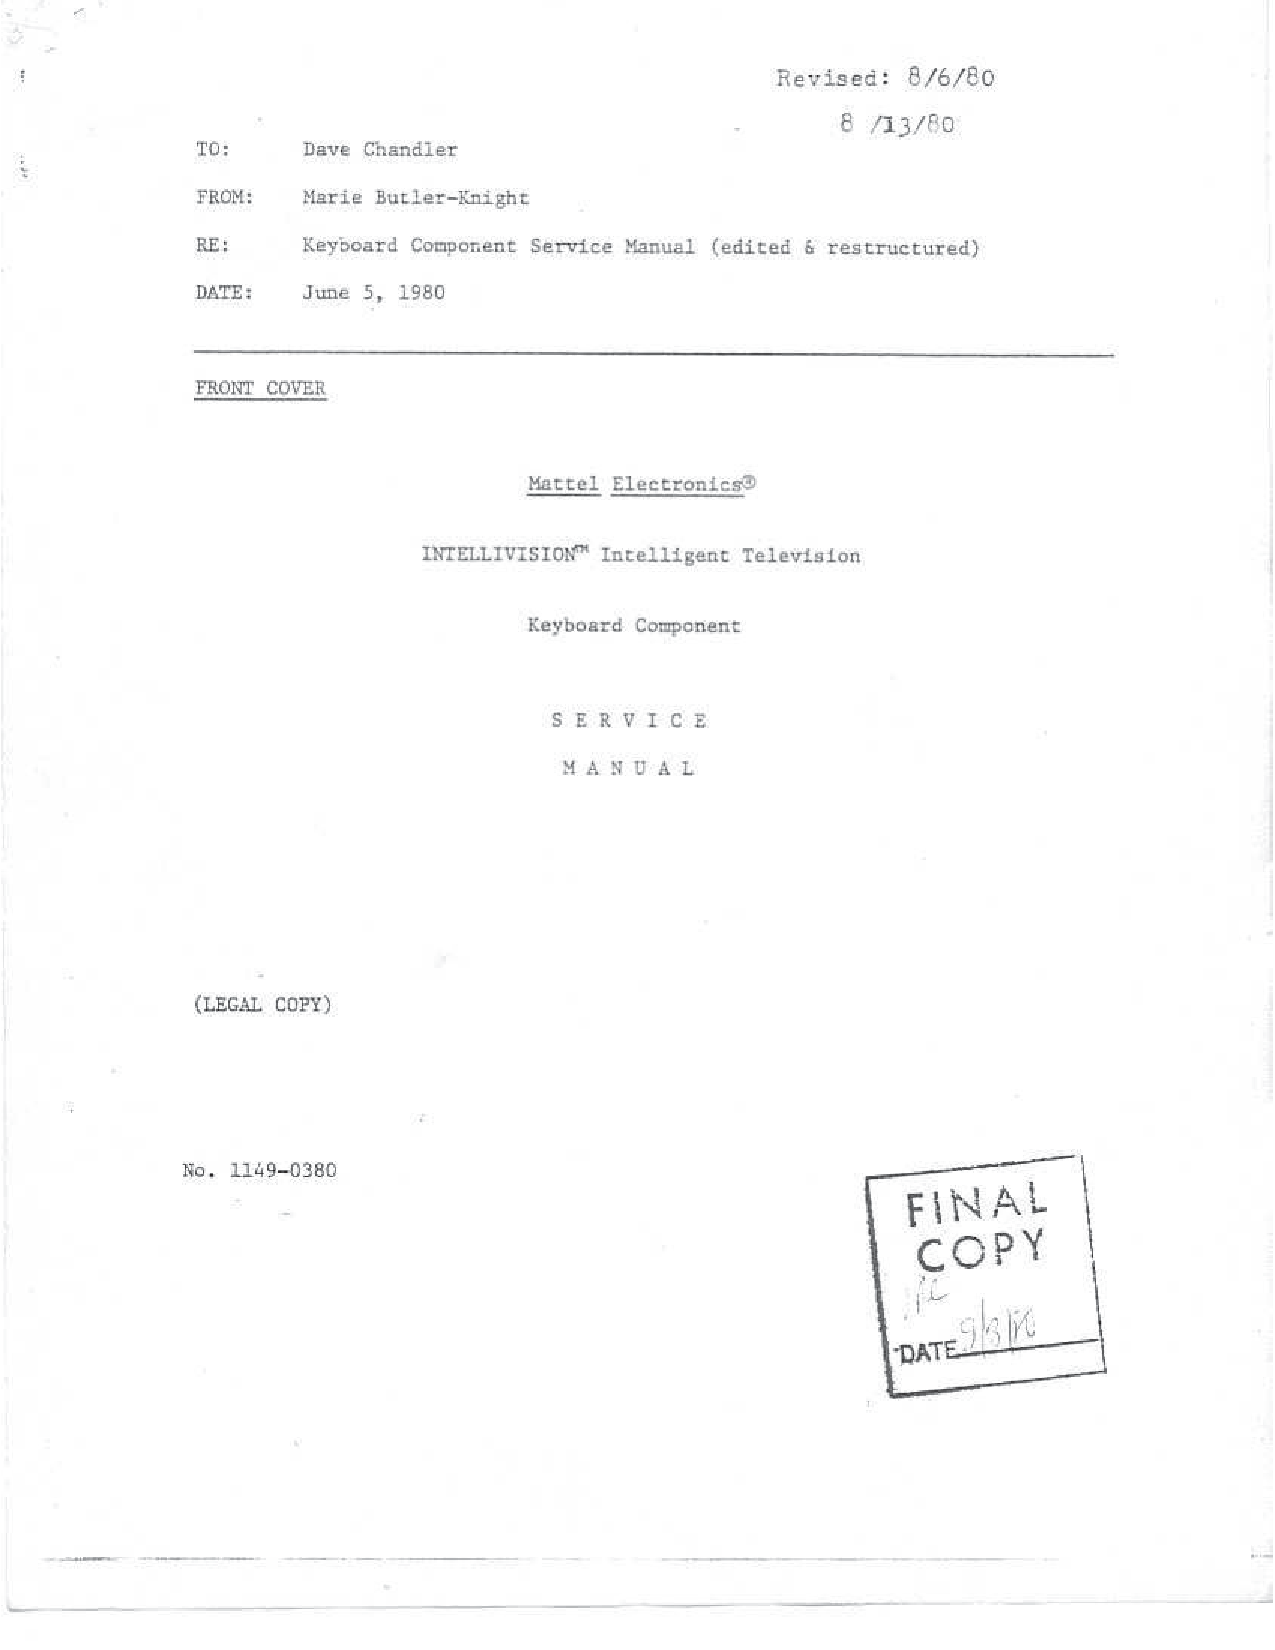
\includepdf[pages=-,pagecommand={},fitpaper=true]{../manuals/Keyboard_Component_Service_Manual.pdf}

\end{document}
